\documentclass[journal]{IEEEtran} % use the `journal` option for ITherm conference style
\IEEEoverridecommandlockouts
% The preceding line is only needed to identify funding in the first footnote. If that is unneeded, please comment it out.
\usepackage{cite}
\usepackage{amsmath,amssymb,amsfonts}
\usepackage{algorithmic}
\usepackage{graphicx}
\usepackage{textcomp}
\usepackage{url}
\usepackage{xcolor}
\usepackage{booktabs}
\usepackage{multirow}
\usepackage{subfig}

\def\BibTeX{{\rm B\kern-.05em{\sc i\kern-.025em b}\kern-.08em
    T\kern-.1667em\lower.7ex\hbox{E}\kern-.125emX}}

\begin{document}

\title{Interpretation of Neural Network Players for a Generalized Divide the Dollar Game Using SHAP Values\\
% delete or comment-out the following line before submission

}

\author{%%%% author names
    \IEEEauthorblockN{G. Greenwood}% first author
    , \IEEEauthorblockN{H. Abbass}% delete this line if not needed
    , \IEEEauthorblockN{A. Hussein}% delete this line if not needed
    % duplicate the line above as many times as needed to list all authors
    \\%%%% author affiliations
    \IEEEauthorblockA{\textit{dept. name of organization (of Aff.), City, Country}}\\% first affiliation
    \IEEEauthorblockA{\textit{dept. name of organization (of Aff.), City, Country if needed}}\\% delete this line if not needed
    % duplicate the line above as many times as needed to list all affiliations
    %%%% corresponding author contact details
    \IEEEauthorblockA{email address or ORCID of corresponding author(s)}
}

\maketitle

\begin{abstract}
    $\cdots$
\end{abstract}

\begin{IEEEkeywords}
    explainable AI, machine learning, model interpretation
\end{IEEEkeywords}

\section{Introduction}

Machine learning (ML) algorithms often operate as black boxes. They receive inputs and render output predictions but often there are questions about how that process works. Explainable AI (abbreviated XAI) is a set of methods that attempt to get some answers.
In previous work~\cite{gree1} we used an evolutionary algorithm to evolve neural network (NN) players for a 3-player game. In this paper we describe how some XAI methods were used to help understand the NN predictions.


Bargaining situations arise whenever two or more people must agree for mutual benefit over some economic transaction. Nash~\cite{nash} created a nonzero-sum two-person game to study bargaining. \textit{Divide the dollar} is a simplified version of Nash's game. Each round two players simultaneously bid on how much of \$1 they are willing to accept. The players get a payoff equal to their bid if the bid total does not exceed \$1; otherwise the players get a zero payoff. In a \emph{generalized divide the dollar} (GDD) game the \$1 is split by $n>2$ players \cite{dan1}. 
%This game has an interesting characteristic: any pair of bids that sum to exactly \$1 is a Nash equilibrium. That is, any player who unilaterally changes his bid cannot improve  his payoff.

We had used a CMA-ES algorithm to evolve NN players for a 3-player GDD game~\cite{gree1}. The input features were the bids of a player's opponents in the previous two rounds. The NN regression output was a player's bid. Three NNs were evolved that were effective and yet exhibited ``fair'' bidding---i.e., the bid total was at or near \$1, but the bids were roughly equal so no player was exploited. Although the NNs performed well, they are still just black boxes. 
It therefore is not possible to explain how they produced a particular prediction (a bid).

\emph{Explainability} and \emph{interpretability} are often used interchangably when talking about ML models but they don't mean the same thing. Explainability tries to understand the inner workings of the ML model. Conversely, interpretability tries to understand what the model considered in making a prediction. For example, consider a deep learning neural network. Explainability might analyze synaptic weights to see how predictions are computed; interpretability would determine which input features were most important in making the predictions. Put another way, explainability tries to determine \emph{how} a model computed a prediction while interpretability tries to determine \emph{why} the prediction was made. Humans are far more interested in interpretability.
There are two types of interpretability:
\begin{itemize}
    \item {\bf Global interpretability:} which input features were most important, over an entire training/test set, in determining the model's outputs.
    \item {\bf Local interpretability:} given a single input, which input features were most important in producing the observed output. 
\end{itemize}


A simple example will help fix ideas. Suppose a bank uses a neural network (NN) to evaluate car loan applicants. The input features are the applicant's profile: age, sex, income, years at current residence and so on. The NN output is the probability the applicant will be make the monthly payments. Alice applies for a loan but is denied because the NN output is 49\%. She asks the loan manager why her application was denied. Explainability would tell which synaptic weights on the hidden layer produced the 49\% prediction. Alice probably wouldn't care about that. But interpretability might determine \verb|age| was the biggest factor in producing a low score. 
In this scenario global interpretability isn't going to be helpful, but local interpretability will provide Alice an answer.


Some ML models, such as linear regession models or tree-based models (e.g., random forest), are interpretable while more complex, black box models such as NNs are not. We need a \textit{model-agnostic} interpretation method that does not require any knowledge about the underlying model. One approach is to construct an \textit{explainer model} that approximates the complex model's predictions (at least for a single input data point $x$). The black box model may not be interpretable, but the explainer model is. If the explainer model's prediction is a good approximation, then interpreting it will also interpret the black box model. Efficient methods exist to extract SHAP values from an explainer model. These SHAP values, which were derived from the game 
theoretical optimal Shapley values, will produce the interpretation.  



The ML model in our work are NNs representing players for a 3-player GDD game. XGBoost \cite{xgb}, a popular ML algorithm, was used for an explainer model. Both global and local interpretations of the model were conducted.

The paper is organized as follows $\ldots$

\section{Background}\label{AA}

\begin{figure}[htbp]
    \centerline{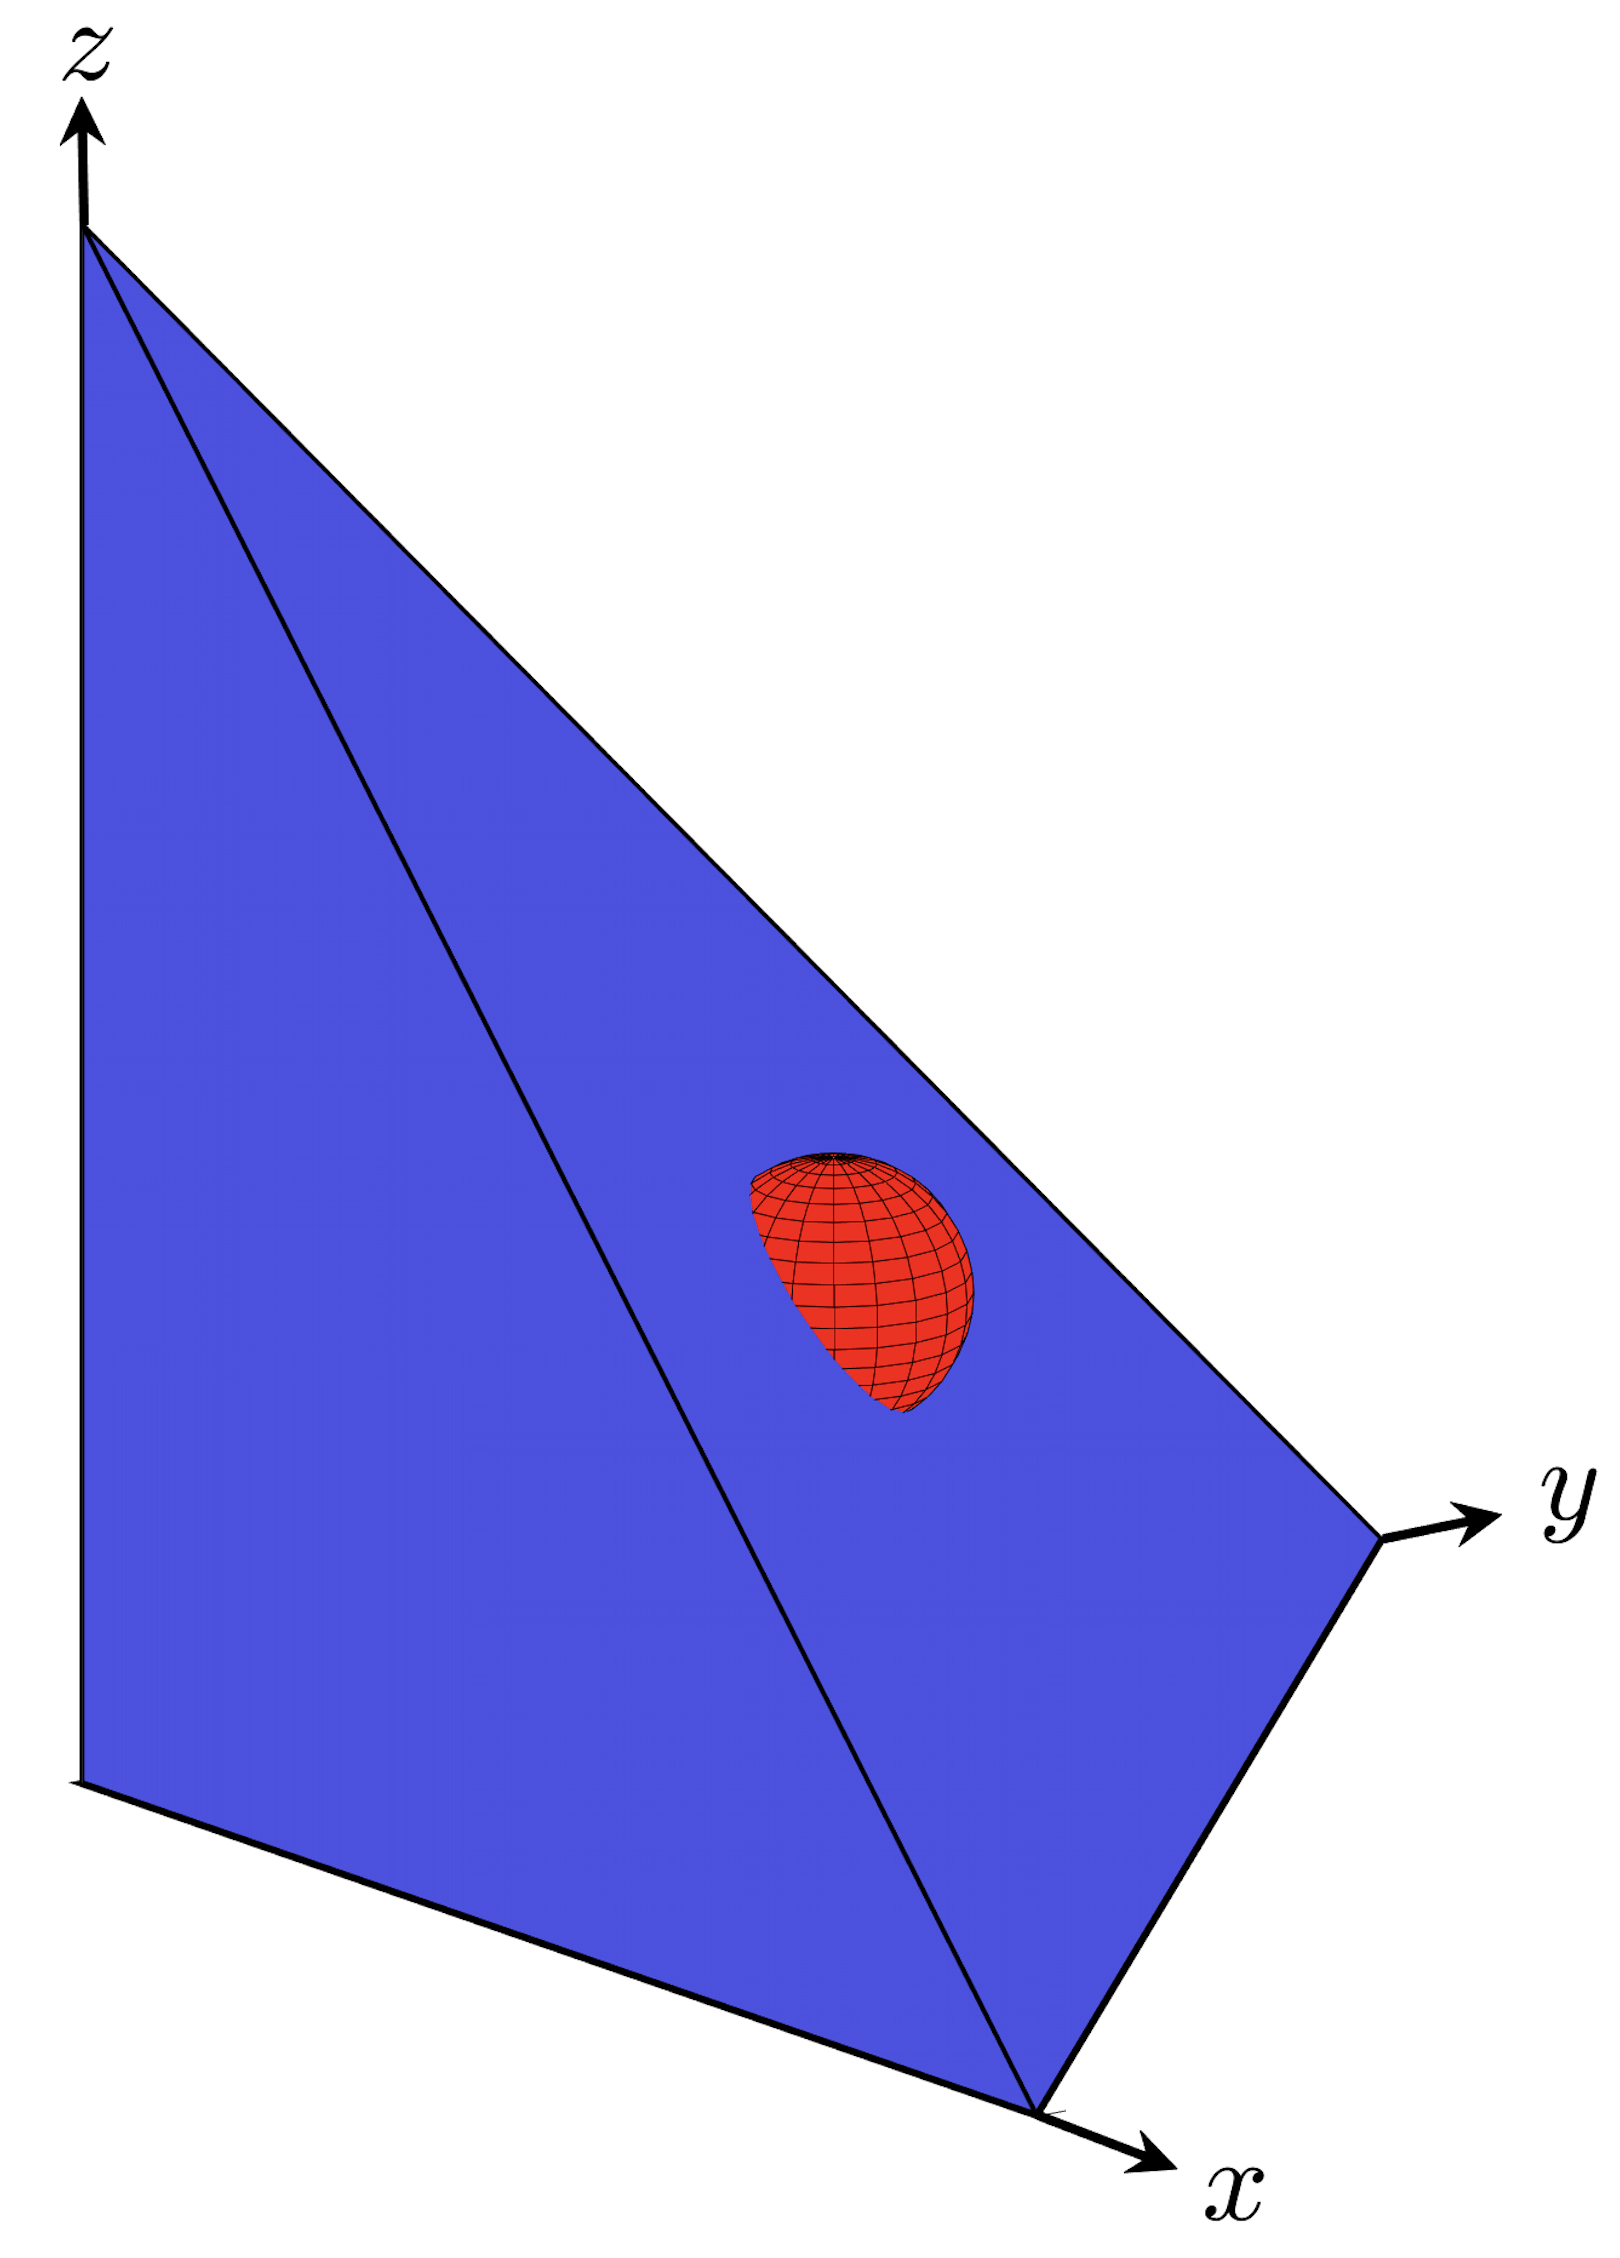
\includegraphics[width=5.2cm]{subsidize.png}}
    \caption{The coordinated subspace for a 3-player GDD game. The subsidy region is the hemisphere protruding from the 2-simplex face.}
    \label{lidija2}
\end{figure}

\subsection{GDD game}

Divide-the-dollar was originally created as a 2-player game. Each round the players would simultaneously submit a bid stating what fraction of a dollar they were willing to accept. If the bid total was a dollar or less the players would get their bid as a payoff. However, if the bid total was over a dollar both players got nothing.

GDD extends the basic divide the dollar game in two ways. First, it is now an $N$-player game with $N>2$. Second, a small subsidy is available. This subsidy allows players to still get a non-zero payoff even if the bid total goes over one dollar. However, the subsidy is available if and only if the bids are ``fair''. That is, no player receives a payoff substantially higher than another player. For example, in a 3-player game with bids of $\{0.61, 0.20, 0.22\}$ the bid total is \$1.03 but one player would receive a much higher payoff. Now suppose the bids were $\{0.33, 0.35, 0.35\}$. Again the bid total is \$1.03, but the payoffs are roughly the same. The subsidy would only be available in the second case.

Bit totals are called \emph{coordinated} if the players receive a non-zero payoff and are called \emph{uncoordinated} otherwise. For an $N$-player game one can think of each bid as a coordinate of a point in $\mathbb{R}^N$. The magnitude of a vector from the origin to this point equals the bid total. Fig.~\ref{lidija2} shows a subspace in $\mathbb{R}^3$. The slanted isosceles triangle is a 2-simplex where all bids total to exactly one dollar. The coordinated bid subspace is the 2-simplex and all points beneath it. 

A hemisphere is shown protruding from the 2-simplex. This hemisphere and its interior represent the subsidy region. Notice it is centered on the 2-simplex at the point the [1/3 1/3 1/3] so only fair bid sets are able to use a subsidy. For $N>3$ players the subsidy region is a hypersphere centered at the point $\left[ \frac{1}{N} \  \frac{1}{N} \  \ldots \  \frac{1}{N} \right]$.



\begin{figure}[htbp]
    \centerline{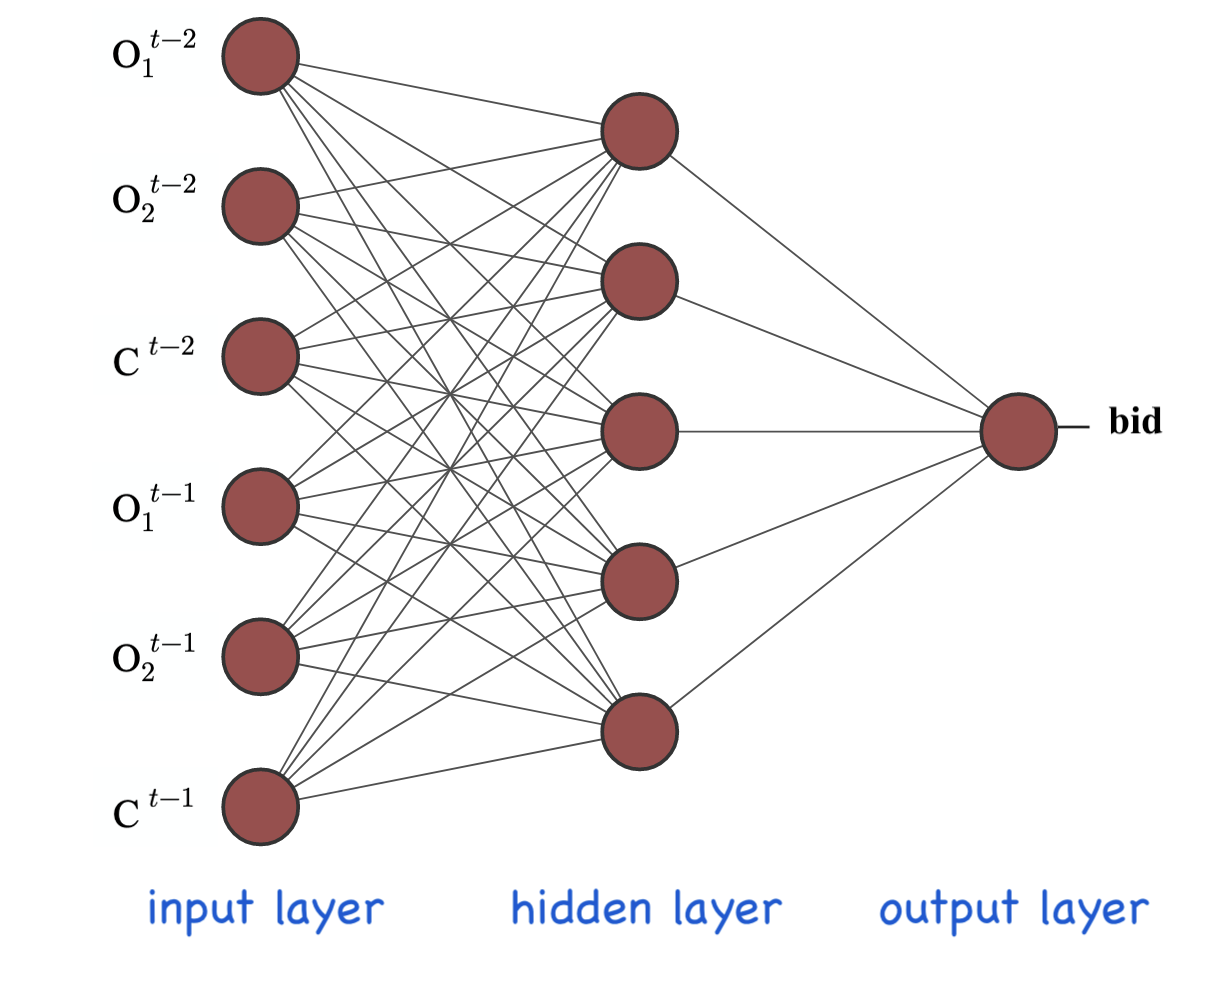
\includegraphics[width=9.1cm]{arch22.png}}
    \caption{The NN architecture for GDD players. See text for notation description.}
    \label{lidija3}
\end{figure}

\subsection{The NN player architecture}

Fig.~\ref{lidija3} shows the architecture of a NN player. At every step $t$ each NN receives 6 input features. Three features are the bids of its two opponents $O_1$ and $O_2$ at time step $t-1$ plus a $C$ input indicating whether the bid total at that time step was coordinated or non-coordinated. ($C$=0.5 if coordinated or 0.0 if non-coordinated.) Another 3 similar set of features are provided for time step $t-2$.  

The NN could have input its own previous outputs instead of $C^{t-1}$ and $C^{t-2}$. However, that would make it difficult to evolve the NN because then it must learn whether or not the previous bids were coordinated. By using the $C$ input method the NN is told if it is coordinated or not. In effect, a $C$ input is similar to the feedback used in reinforcement learning. 


\begin{figure}[tbp]
\centerline{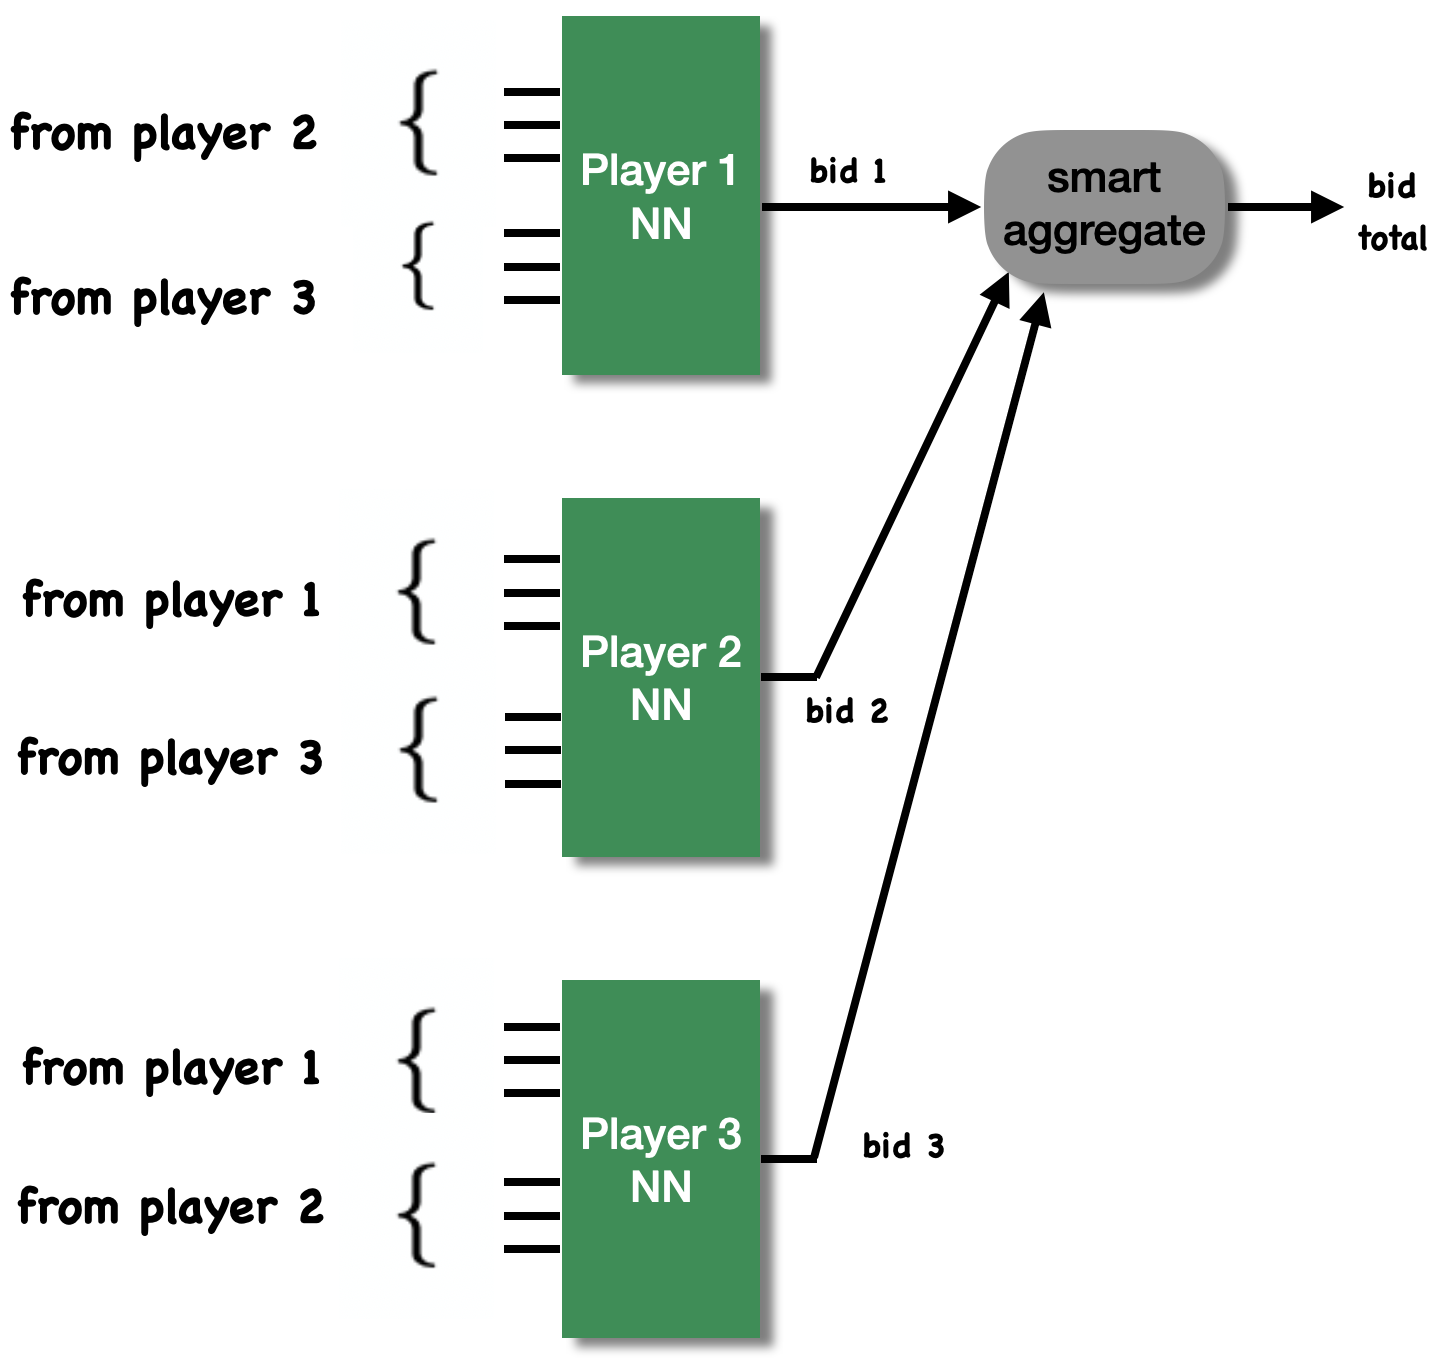
\includegraphics[width=8.7cm,height=9cm]{AMY2.png}}
\caption{The 3-player GDD framework. }
\label{lidija4}
\end{figure}

Fig.~\ref{lidija4} shows the configuration of a 3-player GDD game. Players are represented by a NN with prior bids made by its opponents in previous rounds as feature inputs. Let $b_i$ be the current bid of the $i$-th NN player in an $N$-player game. Each $b_i$ is a coordinate of a point in $\mathbb{R}^N$. The smart aggregator block outputs $\sum_i b_i$ if this point is on or beneath the simplex surface or inside the subsidy hypersphere. Otherwise it outputs 0.

For convenience a special notation was used to label the feature inputs to the NNs. NN2 and NN3 are the 2 opponents of NN1. Consider the following feature vector input to NN1:

\[
\arraycolsep=1.4pt\def\arraystretch{1.2}
\begin{array}{l}
\left\{ \text{O}^{t-2}_{1}\  \text{O}^{t-2}_{2}\  \text{C}^{t-2}\  \text{O}^{t-2}_{1}\  \text{O}^{t-2}_{2}\  \text{C}^{t-1}\right\}  \  =\ \\ 
\hspace{2.2cm} \left\{ \text{O22 O32 C2 O21 O31 C1} \right\} 
\end{array}
\]

 O22 stands for the NN2 bid at time $t-2$.  It is the $O_1^{t-2}$ input in Fig.~\ref{lidija2}.  O32 is the NN3 bid at time $t-2$; it is input $O_2^{t-2}$. C2 is the $C^{t-2}$ input. 
Table \ref{tbl1} lists the input features for each NN.

\begin{table}[htbp]
\caption{Feature inputs for NN players}
\begin{center}
\begin{tabular}{ |c|c| } 
\hline
Neural Network & Input Feature Set  \\
\hline
\multirow{2}*{NN1} & O22, O32, C2 \\ 
& O21, O31, C1  \\ 
\hline
\multirow{2}*{NN2} & O12, O32, C2 \\ 
& O11, O31, C1  \\ 
\hline
\multirow{2}*{NN3} &  O12, O22, C2 \\ 
& O11, O21, C1  \\ 
\hline
\end{tabular}
\end{center}
\label{tbl1}
\end{table}


%\begin{figure}[!t]
%\centerline{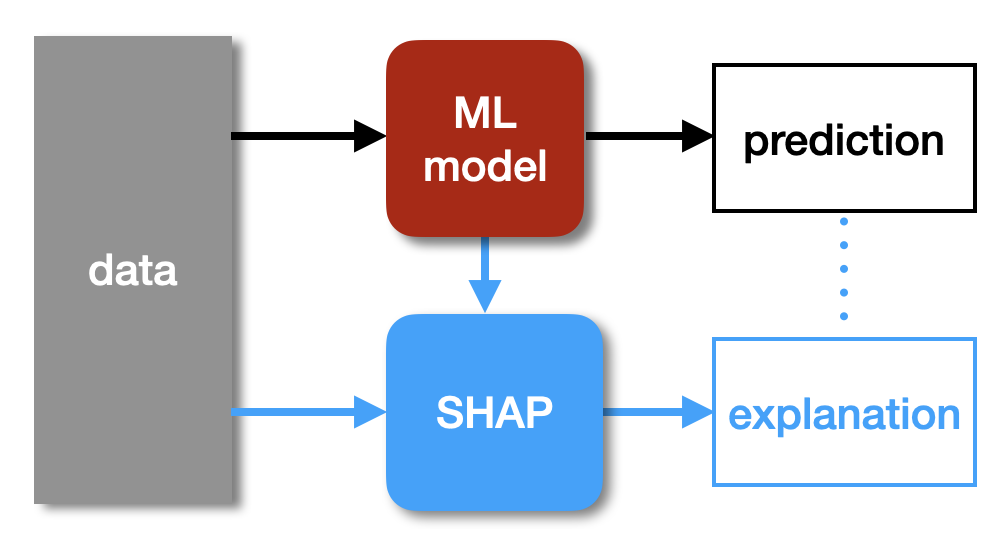
\includegraphics[width=9cm,height=6.3cm]{SHAP.png}}
%\caption{The ML model is a black box. A simpler explainer model is %constructed that approximates the ML model prediction. The explainer model %is interpretable. Since it mimicks the ML model prediction, it can explain %the ML model.}
%\label{lidija22}
%\end{figure}



\subsection{SHAP}

Imagine a game where at the end of each round a payoff is distributed among the players.  How much of the payoff should each player receive? A fair distribution would be based on a player's contribution, but often there are coalitions of players which makes individual contributions not so obvious. Lloyd Shapley~\cite{shapley} answered the question optimally by introducing what are called \emph{Shapley values}. These values specify each player's contribution to a game outcome over all possible player coalitions. In mathematical terms, they are the average marginal contribution over all possible player coalitions. 

Let $\upsilon(S)$ be a characteristic function giving the value of a coalition of players $S$. In a game with $p$ players, the contribution of player $i$ is
\begin{equation}
  \varphi_{i}  =  \sum_{S\subseteq \{1,\ldots p\}\text{} \backslash \left\{ i\right\}  \text{} } \frac{\left| S\right|  !\left( p-\left| S\right|  -1\right)  !}{p!} \left( \upsilon\left( S\cup \left\{ i\right\}  \right)  -\upsilon(S)\right)  
  \label{eqn1}
\end{equation}

The key idea is to determine a player $i$'s contribution $\varphi_i$, one must evaluate the game characteristic function both with and without a player $i$ and then average that over all permutations. Shapley values have several properties:

\begin{itemize}
    \item \textit{Symmetry:} If $\upsilon(S\cup\{i\}) = \upsilon(S\cup\{j\})$ for every coalition $S$, then $\varphi_i=\varphi_j$.
    \item \textit{Dummy:} If $\upsilon(S)=\upsilon(S\cup\{i\})\ \forall S$ not containing $i$, then $\varphi_i=0$.
    \item \textit{Additivity:} Let $\upsilon$ and $u$ be two distinct characteristic functions. Then $\varphi^{\upsilon +u}_{i} =\  \varphi^{\upsilon }_{i} +\varphi^{u}_{i}$ 
\end{itemize}
\vspace{1ex}

Lundberg and Lee~\cite{lund} introduced a method called SHapley Additive exPlanations (or SHAP) to interpret ML black box models through Shapley values. Games now become ML models, players now become input features and characteristic functions now become model predictions. 

In KernelSHAP, which is model-agnostic, local interpretation is done by taking a single observation from the database and checking how the model prediction changes with samples of coalitions (subsets) of the features. In some coalitions features may be missing. A weighted linear model is fit to these sample coalitions and the coefficients are the Shapley values.
With $M$ input features there are $M$ SHAP values 
$\left\{ \phi_{1} \  \phi_{2} \  \cdots \  \phi_{M} \right\}$. Each $\phi_i$ is the average marginal contribution of that feature among all sampled coalitions. 

\begin{equation}
    \phi_{i} \  =\  \begin{gathered}\text{Average over sampled}\\ \text{features}^{\prime }  \text{subsets}\\ \text{S} \subseteq \text{M} \backslash \{i\} \end{gathered} \  \left( f(\text{S} \cup \{ i\} \right)  -f\left( \text{S} \right)  )\label{eqn2}
\end{equation}

\noindent where $f(S)$ is the model's prediction for some coalition of features $S$.
SHAP values have an additive attribution property. That is, the sum of the SHAP values equals the final prediction\footnotemark.

\begin{equation}
f(x) = E\left[ f(x)\right]  +\sum^{M}_{i=1} \phi_{i}
    \label{eqn3}
\end{equation}

\footnotetext{Equation \eqref{eqn3} assumes all features are present in the data point.}


Equations \eqref{eqn1} and \eqref{eqn2} are computationally expensive. SHAP is actually an open-source library that efficiently computes Shapley values in ML domains. It contains algorithms to find exact Shapley values for tree ensemble models (TreeSHAP), and approximate Shapley values for deep learning models (DeepSHAP). KernelSHAP is model-agnostic because it can approximate Shapley values for any type of model. Further details can be found in~\cite{tree, shap}.

\section{Results}

In this section both local and global interpretations of the player NNs are presented. XGBoost, which is a gradient boosting algorithm, was the ML model to be interpreted. Since this is a tree ensemble model TreeSHAP extracted the SHAP values. One thousand trees were involved with a tree depth of 5 and a learning rate of $\eta=0.02$. The maximum available subsidy was \$0.05.
Three feature vectors are chosen for local interpretation: one for a coordinated bid with a bid total less than or equal to 1, a subsidized bid, and an uncoordinated bid. Decision plots are used to show the results.

In decision plots the input features are listed from top to bottom in order of importance---i.e., the top feature had the greatest impact on the model prediction. A vertical line shows the baseline value. This is the output of a model with no input features; it is the average model prediction in the training set. The raw feature value is shown in parenthesis.  SHAP is an additive attribution method so adding a feature increases or decreases the prediction relative to the baseline value. A segmented line shows how each SHAP value adds to the prediction. The final prediction is where this segmented line intersects the number line at the top of the plot. Blue lines indicate a final prediction lower than the baseline and red lines higher than the baseline. 

It is interesting to see the interaction between players. Players try to get coordinated bid totals because otherwise there is no payoff. Consequently, opponent bids above the baseline in previous rounds tend to drive current bids lower. Players can be altruistic. Low opponent bids have the opposite effect. Players can also be exploitative. 


Fig.~\ref{amy1} shows decision plots of the three NNs for a randomly chosen coordinated bid total feature vector. All three NNs had predictions below the baseline value. NN1 considered opponent bids in the previous round as important, and, since those bids are high, the final prediction is low. For NN2 the large bid from NN3 in the previous round drove the prediction lower but the below baseline NN1 bid drove it higher. The NN3 output bid consistently moved lower except the low bid from NN1 in the previous round drove it to a higher final prediction. 

Low opponent bids in previous rounds tends to increase the bid in the current round. Fig.~\ref{amy2} shows an uncoordinated bid decision plot.  At this data point all 3 NNs saw low opponent bids in previous rounds and so significantly increase their bid. Such behavior increases the likelihood of uncoordinated bid totals. 

Decision plots for a subsidized bid total are shown in Fig.~\ref{amy3}. NN1 dramatically increased its bid because the input features indicated the other opponent bids were low in the previous two rounds and the bid totals were coordinated. NN2 and NN3 had similar behavior. Both would have had a high bid if it were not for the very high NN1 bid in the previous round. Indeed, O11 was the most influential feature for both NNs. 

A global interpretation is depicted in Fig.~\ref{amy4}. The beeswarm plot shows all three NNs see the opponent's bids in the previous round ($t-1$) have the most influence on current predictions. Notice the red portion is to the left for all $Oij$ bid inputs but to the right on all $Cj$ inputs. High opponent bids lead to lower current bids which promotes altruistic behavior. Conversely, coordinated bids in the previous rounds tend to increase the current bid. This could explain the exploitative behavior. Opponent bids in earlier rounds ($t-2$) have the least effect on current bids.

\begin{figure}[!t]
\centerline{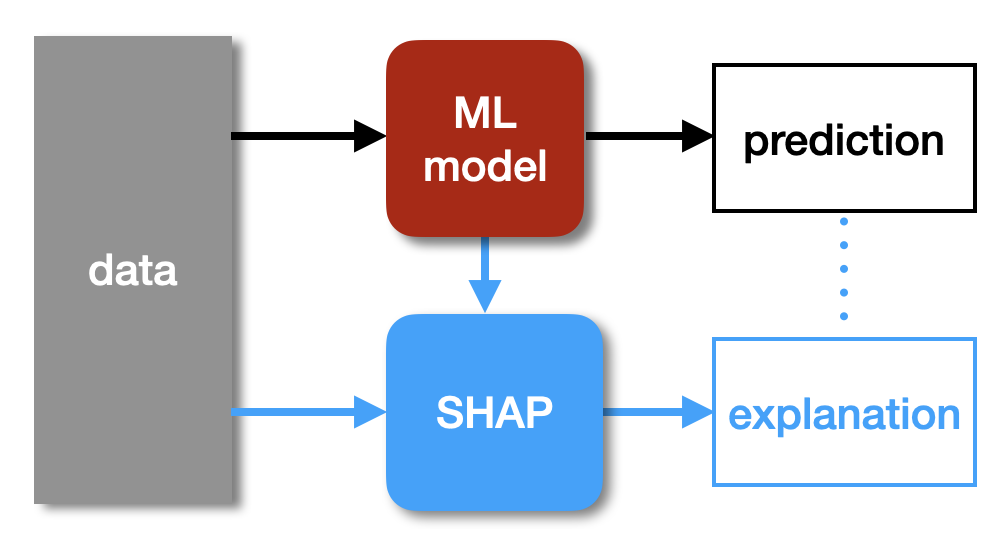
\includegraphics[width=8.2cm,height=4.3cm]{SHAP.png}}
\caption{The SHAP framework.}
\label{lidija1}
\end{figure}

\section{Discussion}

The goal is to explain why NN players make particular bids. Fig.~\ref{lidija1} shows the SHAP framework used for model explanation. The ML model is first fit to a database. Then observations from the database and the model are fed to SHAP which computes $\phi_i$ for each feature $i$. Equation~\eqref{eqn3} provides the explanation. 

Unfortunately we could not just substitute a player's NN for the ML model.  Our problem is no database is available. Usually NNs are trained with a database but in this case they were designed through a cooperative, co-evolutionary process. A CMA-ES algorithm evolved the NN synaptic weights and fitness was determined via a series of 15 round tournaments against other NN players. (See \cite{gree2} for details.) 

A process similar to creating global surrogate models was used to build a database.
An observation was constructed by applying random inputs to a NN player and recording the prediction (a bid). The baseline bid for the three players was [1/3 1/3 1/3]. Random noise was then added to the baseline to get feature vectors. For example, referring to Fig.~\ref{lidija3}, 
\[
O_1^{t-1} = 1/3 + \mathcal{N}(0,\sigma)
\]
\noindent where $\mathcal{N}(0,\sigma)$ is a normally distributed random variable with zero mean and standard deviation $\sigma$. In this work $\sigma=0.025$ is used. Other features are computed similarly. The $C_1$ and $C_2$ values are set since all NN outputs at $t-1$ and $t-2$ are known. This process was repeated to build a database with 2000 observations.

The ML model shown in Fig.~\ref{lidija1} was XGBoost. Effectively it is a global surrogate model. An R$^2=0.996$ value indicates the XGBoost model adequately approximates the NN model. Thus, any assumptions made about the XGBoost model holds for the NN model. TreeSHAP can efficiently extract the SHAP values from boosted tree models. 

\vspace{0.2cm}
***********
\textcolor{blue}{more yet to be added}
***********
\section{Final Remarks}
 \begin{figure*}[!bt]
    \centering
    \subfloat[NN1]{%
      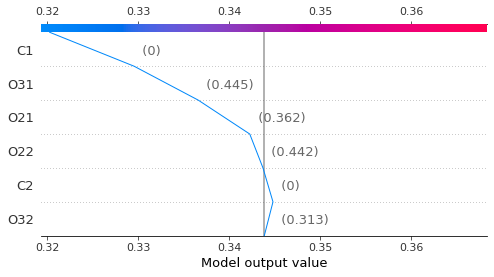
\includegraphics[width=5.8cm,height=4cm]{1c.png}
    }
    \subfloat[NN2]{%
            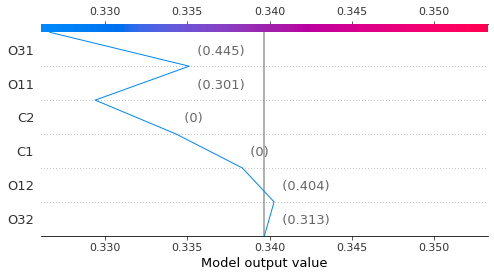
\includegraphics[width=5.8cm,height=4cm]{2c.png}
            }
    \subfloat[NN3]{%
            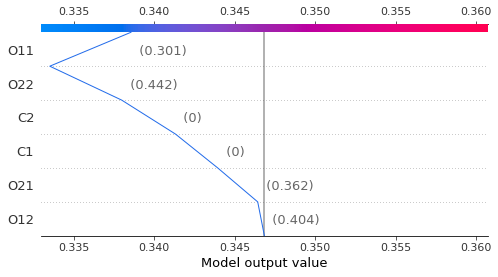
\includegraphics[width=5.8cm,height=4cm]{3c.png}
            }
    \caption{Decision plots for a coordinated bid total.}\label{fig:dummy}
    \label{amy1}
  \end{figure*}

 \begin{figure*}[!bt]
    \centering
    \subfloat[NN1]{%
      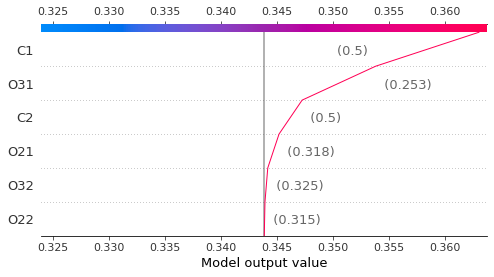
\includegraphics[width=5.8cm,height=4cm]{1u.png}
    }
    \subfloat[NN2]{%
            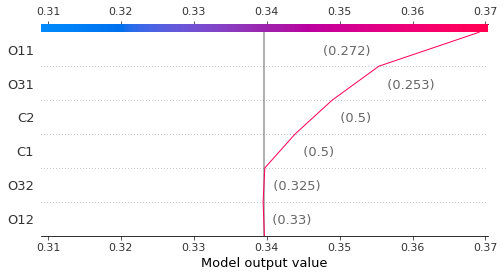
\includegraphics[width=5.8cm,height=4cm]{2u.png}
            }
    \subfloat[NN3]{%
            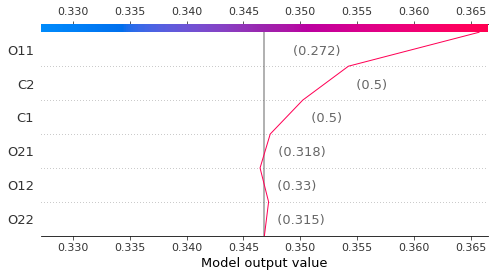
\includegraphics[width=5.8cm,height=4cm]{3u.png}
            }
    \caption{Decision plots for an uncoordinated bid total.}\label{amy2}
\end{figure*}

\begin{figure*}[!bt]
    \centering
    \subfloat[NN1]{%
      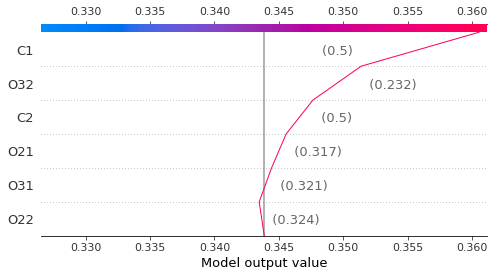
\includegraphics[width=5.8cm,height=4cm]{1s.png}
    }
    \subfloat[NN2]{%
            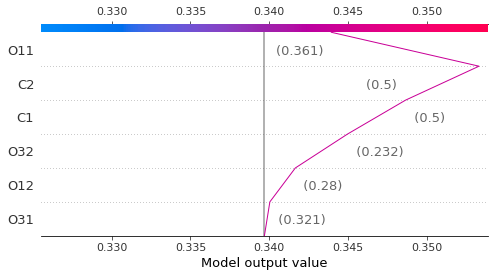
\includegraphics[width=5.8cm,height=4cm]{2s.png}
            }
    \subfloat[NN3]{%
            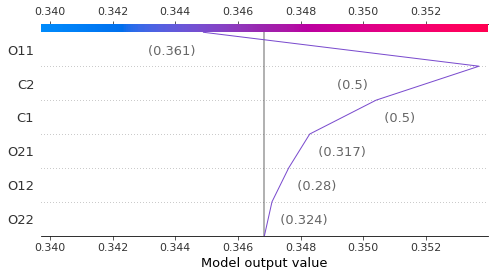
\includegraphics[width=5.8cm,height=4cm]{3s.png}
            }
    \caption{Decision plot for a subsidized bid total.}\label{amy3}
\end{figure*}

\begin{figure*}[!bt]
    \centering
    \subfloat[NN1]{%
      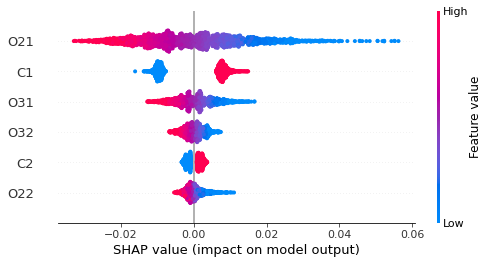
\includegraphics[width=5.8cm,height=4cm]{1b.png}
    }
    \subfloat[NN2]{%
            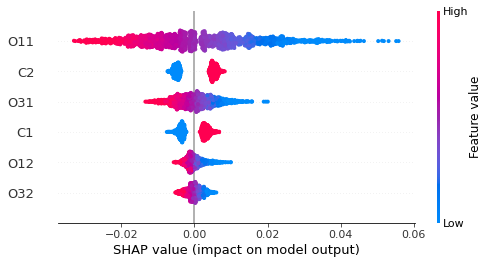
\includegraphics[width=5.8cm,height=4cm]{2b.png}
            }
    \subfloat[NN3]{%
            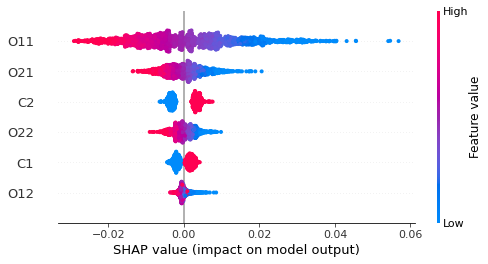
\includegraphics[width=5.8cm,height=4cm]{3b.png}
            }
    \caption{Beeswarm plots showing global interpretation of the three NNs. }\label{amy4}
  \end{figure*}

\newpage
  
\bibliographystyle{unsrt}
\bibliography{cog2021}

\end{document}

%\begin{table}[htbp]
%    \caption{Table Type Styles}
%    \begin{center}
%        \begin{tabular}{|c|c|c|c|}
%            \hline
%            \textbf{Table} & \multicolumn{3}{|c|}{\textbf{Table Column Head}}               %                                          \\
%            \cline{2-4}
%            \textbf{Head}  & \textbf{\textit{Table column subhead}}           & \textbf{\textit{Subhead}} & \textbf{\textit{Subhead}} \\
%            \hline
%            copy           & More table copy$^{\mathrm{a}}$                   &             %              &                           \\
%            \hline
%            \multicolumn{4}{l}{$^{\mathrm{a}}$Sample of a Table footnote.}
%        \end{tabular}
%        \label{tab1}
%    \end{center}
%\end{table}
